\documentclass[12pt,a4paper]{report}
\usepackage{a4wide}
\usepackage[portuguese,english]{babel}
\usepackage{graphics}
\usepackage{amsmath}
\usepackage{epsfig}
\usepackage[latin1]{inputenc}
\usepackage{doublespace}
\usepackage{fancyheadings}
\usepackage{longtable}
\usepackage{dropping}
\usepackage{url}
\usepackage{subfigure}
\usepackage[top=3cm,left=3cm,bottom=2cm,right=2cm]{geometry}


%\usepackage{apalike}
\newcommand{\figr}[1]{Figura~\ref{#1}}
\newcommand{\eqt}[1]{Eq.~(\ref{#1})}
\newcommand{\eqts}[2]{Eq.~(\ref{#1})~e~(\ref{#2})}
\newcommand{\eqtss}[3]{Eq.~(\ref{#1})~,~(\ref{#2})~e~(\ref{#3})}
\newcommand{\tab}[1]{Tabela~\ref{#1}}

%comandos para se definir cabe�alhos nas p�ginas da disserta��o
\pagestyle{fancyplain}
\lhead[\fancyplain{}{\thepage}]{\fancyplain{}{\small\leftmark}}
\rhead[\fancyplain{}{\small\rightmark}]{\fancyplain{}{\thepage}}
\cfoot{\fancyplain{\thepage}{}}

%package para reconhecimento de acentua��o em portugu�s
\usepackage[latin1]{inputenc}

%package para reconhecimento de portugu�s
\usepackage{babel}

%package para uso de verbatimtab
%\usepackage{moreverb}

%configura��o para numera��o de subsubse��es
\setcounter{secnumdepth}{3}

% Frases de efeito no in�cio de cada cap�tulo
\newcommand{\epigraph}[2]{%
  \vspace{1ex}%
  {\footnotesize%
   \begin{spacing}{1}
    \begin{flushright}%
      \begin{minipage}{.6\textwidth}%
        #1\\
      \end{minipage}\\
      \textit{#2}%
    \end{flushright}
    \end{spacing}}%
  \vspace{1ex}}



\begin{document}

%-----------------------------------
% CAPA EM PORTUGU�S
%-----------------------------------
\thispagestyle{empty}

\begin{spacing}{1.0}

\begin{center}
\begin{large}
\begin{huge}
CENTRO UNIVERSIT�RIO DA FEI\\[0.2 cm]
\end{huge}

\vspace {2 cm}


MAUR�CIO KENITI HIROTA\\[0.2 cm]

FABR�CIO LOPES DE SOUZA\\[0.2 cm]

IVAN SHIGUENORI MACHIDA\\[0.2 cm]

THIAGO MIZUTANI\\[0.2 cm]

Orientador: Prof. D.Sc. Paulo S�rgio Silva Rodrigues \\[0.2 cm]
\end{large}
\end{center}

\vspace {2 cm}

\begin{spacing}{1.5}
\begin{center}
\begin{huge}
{\bf MANUAL DE USO - M-FIT}
\end{huge}
\end{center}
\end{spacing}

\vspace {8 cm}

\begin{center}
\begin{large}
S�o Bernardo do Campo \\[0.2 cm]
2008
\end{large}
\end{center}

\end{spacing}
\newpage

%-----------------------------------
% CAPA DE APRESENTA��O EM PORTUGU�S
%-----------------------------------
\thispagestyle{empty}

\begin{spacing}{1.0}

\begin{center}
\begin{large}
\begin{huge}
CENTRO UNIVERSIT�RIO DA FEI\\[0.2 cm]
\end{huge}

\vspace {2 cm}

MAUR�CIO KENITI HIROTA\\[0.2 cm]

FABR�CIO LOPES DE SOUZA\\[0.2 cm]

IVAN SHIGUENORI MACHIDA\\[0.2 cm]

THIAGO MIZUTANI\\[0.2 cm]

Orientador: Prof. D.Sc. Paulo S�rgio Silva Rodrigues \\[0.2 cm]
\end{large}
\end{center}

\vspace {2 cm}

\begin{spacing}{1.5}
\begin{center}
\begin{huge}
{\bf MANUAL DE USO - M-FIT}

\end{huge}
\end{center}
\end{spacing}

\vspace {2 cm}

\begin{flushright}
\begin{minipage}[t]{8.5 cm}
Trabalho de Conclus�o de Curso, apresentado no Centro Universit�rio
da FEI, como parte dos requisitos necess�rios para obten��o do
t�tulo de Bacharel em Ci�ncias da Computa��o, orientado pelo
professor Prof. D.Sc. Paulo S�rgio Silva Rodrigues.
\end{minipage}
\end{flushright}

\vspace {2 cm}

\begin{center}
\begin{large}
S�o Bernardo do Campo \\[0.2 cm]
2008
\end{large}
\end{center}

\end{spacing}
\newpage


%-----------------------------------
% DOCUMENTA��O DO TRABALHO
%-----------------------------------

\renewcommand{\baselinestretch}{1.3}

\pagenumbering{roman}
%\setlength{\voffset}{0.0in}

%\begin{spacing}{1.0}
%\chapter*{\centering RESUMO \label{resumo}}

\hspace*{1.25cm}Na �rea de Editora��o de V�deos, uma das atividades
mais demandadas � a detec��o de transi��o de tomadas, que �
basicamente a concatena��o do final de uma tomada com o in�cio de
outra. Essa tarefa tem v�rias utilidades em diversas aplica��es,
como indexa��o, recupera��o, an�lise e edi��o de v�deos. Estas
transi��es podem ocorrer de diversas formas, tais como: cortes,
\textit{fades} ou \textit{dissolve}. Este trabalho apresenta o
M-FIT, um \textit{framework} que possibilitar� o reconhecimento autom�tico
das transi��es de tomadas de cenas a partir de uma determinada
amostragem de imagens (\textit{frames} de um v�deo) atrav�s do uso de
t�cnicas de Ritmo Visual e Segmenta��o de Imagens. O M-FIT permite ao usu�rio
aplicar efeitos b�sicos de edi��o de imagens no v�deo, de forma
r�pida e simples. Sua interface � baseada em QT, o que torna o M-FIT
um sistema com uma interface simples e de f�cil entendimento.

%\end{spacing}

%\begin{spacing}{1.0}
%\chapter*{\centering ABSTRACT \label{abstract}}

\hspace*{1.25cm}In the field of Video Editing, the main goal is
detecting take transitions, which is basically the connection of the
end of one take to the begining of the next. This work have much
utilities in many applications, such as indexing, recovering,
analysing and video editing. These transitions can occur in several
ways, such as: cuts, fades, and dissolve. This work presents the
M-FIT, a framework that will let the automatic detection of take
transitions from a sample of images (frames of a video) using
techniques based on Visual Rhythm and image segmentation. The M-FIT
allows the user to apply basic effects in the video, so quick and
simple. Your interface is made with QT, making M-FIT a system with a
simple interface and easy for all users.

%\end{spacing}

\selectlanguage{portuguese}

\begin{spacing}{1.0}
\renewcommand{\contentsname}{Sum�rio}\tableofcontents
%\listoffigures
%\listoftables
\end{spacing}

\clearpage

\setcounter{page}{0} \pagenumbering{arabic}

% Aqui entram todos os t�picos
\begin{spacing}{1.5}

\chapter{Conhecendo os Menus do Sistema \label{menus_do_sistema}}

\hspace*{1.25cm}Neste cap�tulo ser�o apresentados os menus do
sistema, com suas devidas funcionalidades.

\section{Arquivo \label{menu_arquivo}}

\hspace{1.25cm}Neste menu existem as seguintes op��es:

\begin{figure}[h|top]
 \centering
 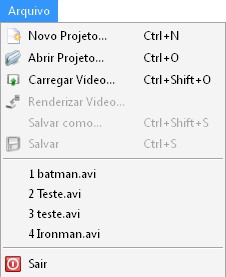
\includegraphics[width=0.5\linewidth]{imagens/menu_arquivo.png}
 \caption{Menu Arquivo.}
 Fonte: Autor.
 \label{img:menu_arquivo}
\end{figure}

\begin{enumerate}

\item{\textbf{Novo Projeto     :} Cria um novo projeto.}
\item{\textbf{Abrir Projeto    :} Abre um projeto j� existente. S�o aceitos somente arquivos com a extens�o MFIT. }
\item{\textbf{Carregar Video   :} Carrega o V�deo desejado. Ap�s o carregamento, a Timeline ser� criada, e v�rias op��es
estar�o habilitadas para uso. S�o aceitos somente arquivos com a extens�o AVI.}
\item{\textbf{Renderizar Video :} Renderiza o V�deo corrente, aplicando nele todos os efeitos definidos pelo usu�rio. Esta op��o s� estar� habilitada no momento em que um V�deo for carregado.}
\item{\textbf{Salvar Como      :} Salva o projeto corrente em arquivo. Todas as altera��es do usu�rio ficar�o salvas para
uso futuro. Esta funcionalidade requisita o nome de projeto ao usu�rio. Esta op��o s� estar� habilitada no momento em que um V�deo for carregado.}
\item{\textbf{Salvar           :} Salva o projeto corrente, caso um nome j� esteja definido, o projeto � salvo sem requisitar um nome de projeto. Esta op��o s� estar� habilitada no momento em que um V�deo for carregado.}
\item{\textbf{Arquivos Recentes:} O espa�o entre os 2 limitadores � reservado para os �ltimos arquivos abertos, sejam eles de
v�deo ou de projeto. }
\item{\textbf{Sair             :} Fecha o MFIT.}

\end{enumerate}

\section{Detec��o \label{menu_deteccao}}

\hspace{1.25cm}Este menu s� tem suas op��es habilitadas para uso se existir um V�deo carregado.
Neste menu existem as seguintes op��es:

\begin{figure}[h|top]
 \centering
 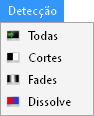
\includegraphics[width=0.2\linewidth]{imagens/menu_deteccao.png}
 \caption{Menu Detec��o.}
 Fonte: Autor.
 \label{img:menu_deteccao}
\end{figure}

\begin{enumerate}

\item{\textbf{Todas   :} Inicia o processo de detec��o de todas as transi��es: Corte, Fade e Dissolve. }
\item{\textbf{Corte   :} Inicia o processo de detec��o de transi��es do tipo Corte. }
\item{\textbf{Fade    :} Inicia o processo de detec��o de transi��es do tipo Fade. }
\item{\textbf{Dissolve:} Inicia o processo de detec��o de transi��es do tipo Dissolve.}

\end{enumerate}

\section{Configura��es \label{menu_configuracoes}}

\hspace{1.25cm}Neste menu existem as seguintes op��es:

\begin{figure}[h|top]
 \centering
 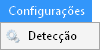
\includegraphics[width=0.2\linewidth]{imagens/menu_configuracoes.png}
 \caption{Menu Configura��es.}
 Fonte: Autor.
 \label{img:menu_configuracao}
\end{figure}

\begin{enumerate}

\item{\textbf{Detec��es :} Abre a janela de configura��es espec�ficas para cada tipo de transi��o }

\end{enumerate}

\section{Barra de Bot�es \label{barra_de_botoes}}

\hspace{1.25cm}Logo abaixo dos menus do sistema se encontra a barra de bot�es.
Esta barra � uma extens�o de todos os menus, sendo que cada bot�o, tem uma entrada correspondente em algum dos menus.
Esta barra proporciona f�cil acesso a op��es dos menus existentes.

\begin{figure}[h|top]
 \centering
 
\includegraphics[width=0.5\linewidth]{imagens/barra_botoes.png}
 \caption{Barra de Bot�es.}
 Fonte: Autor.
 \label{img:barra_botoes}
\end{figure}

\hspace{0.65cm}Da esquerda para a direita, temos:

\begin{enumerate}

\item{\textbf{Novo Projeto}}
\item{\textbf{Abrir Projeto}}
\item{\textbf{Carregar V�deo}}
\item{\textbf{Salvar}}
\item{\textbf{Renderizar V�deo}}
\item{\textbf{Carregar V�deo}}

\item{\textbf{Detec��o de transi��o: Todas}}
\item{\textbf{Detec��o de transi��o: Corte}}
\item{\textbf{Detec��o de transi��o: Fade}}
\item{\textbf{Detec��o de transi��o: Dissolve}}

\item{\textbf{Configura��es: Detec��o}}

\end{enumerate}

\hspace{0.65cm}Note que os �cones destes bot�es s�o os mesmos
utilizados nos menus.

\chapter{Funcionalidades do M-FIT\label{introducao}}

\hspace*{1.25cm}Neste cap�tulo ser� explicado todas as funcionalidades do MFIT.

\section{Carregar um V�deo\label{carrega_video}}

\hspace{1.25cm}Nesta se��o detalharemos os passos necess�rios para
se carregar um V�deo.

\begin{enumerate}

\item{Abra o MFIT (Figura \ref{img:mfit_aberto})}

\begin{figure}[h|top]
 \centering
 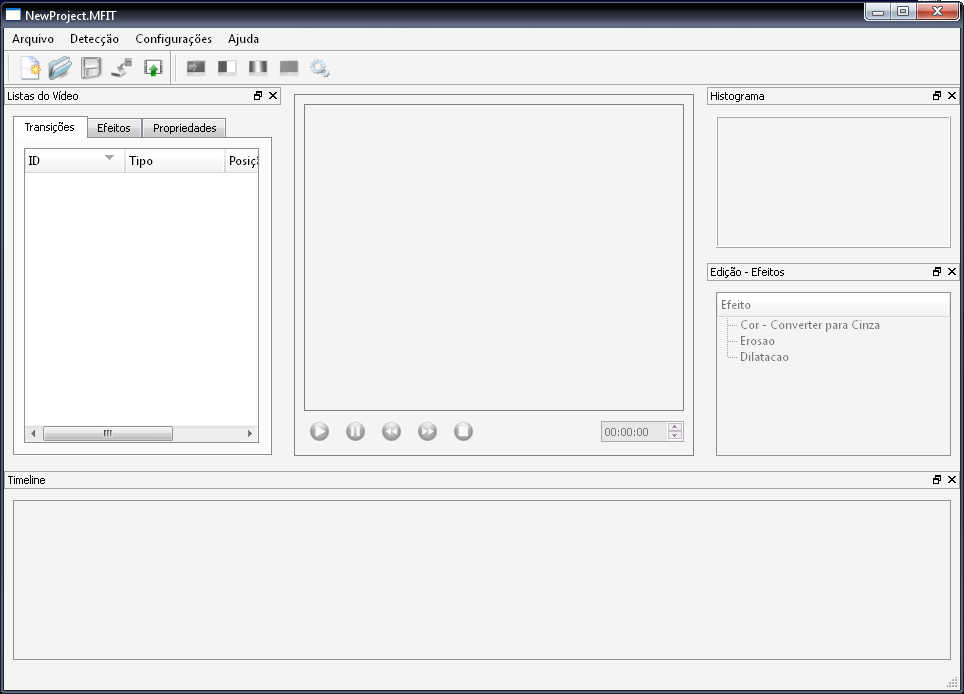
\includegraphics[width=0.7\linewidth]{imagens/mfit_aberto.png}
 \caption{MFIT Aberto sem V�deo carregado.}
 Fonte: Autor.
 \label{img:mfit_aberto}
\end{figure}

\item{Clique com o bot�o direito no menu ``Arquivo'', op��o ``Carregar V�deo''.
Se preferir, pressione as teclas Ctrl+Shif+O (Figura \ref{img:carregar2}). }

\begin{figure}[h|top]
 \centering
 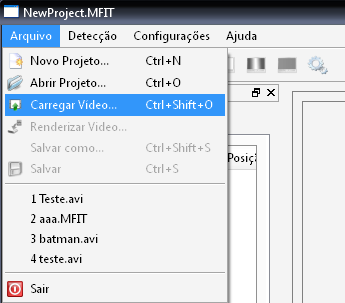
\includegraphics[width=0.7\linewidth]{imagens/carregar2.png}
 \caption{Menu ``Arquivo'', op��o ``Carregar V�deo'' .}
 Fonte: Autor.
 \label{img:carregar2}
\end{figure}

\item{Na janela que abrir�, selecione um V�deo v�lido (com extens�o .AVI) e de um duplo clique (Figura \ref{img:carregar3}). }

\begin{figure}[h|top]
 \centering
 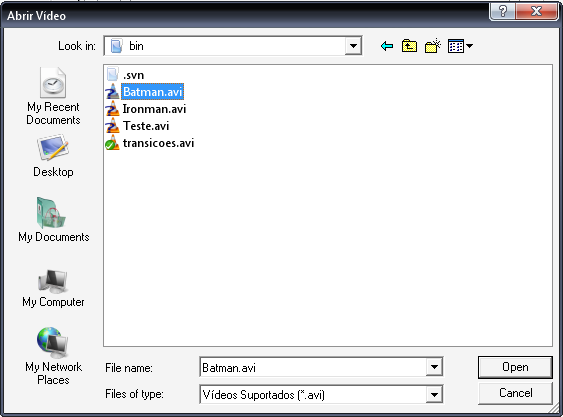
\includegraphics[width=0.7\linewidth]{imagens/carregar3.png}
 \caption{Selecionando um V�deo v�lido.}
 Fonte: Autor.
 \label{img:carregar3}
\end{figure}

\item{Ap�s alguns instantes o v�deo estar� aberto, e sua timeline estar� montada.
Note que uma janela se abrir�, questionando se o processo de detec��o de transi��es deve ser iniciado.
Por hora, clique em cancelar (Figura \ref{img:carregar4}). }

\begin{figure}[h|top]
 \centering
 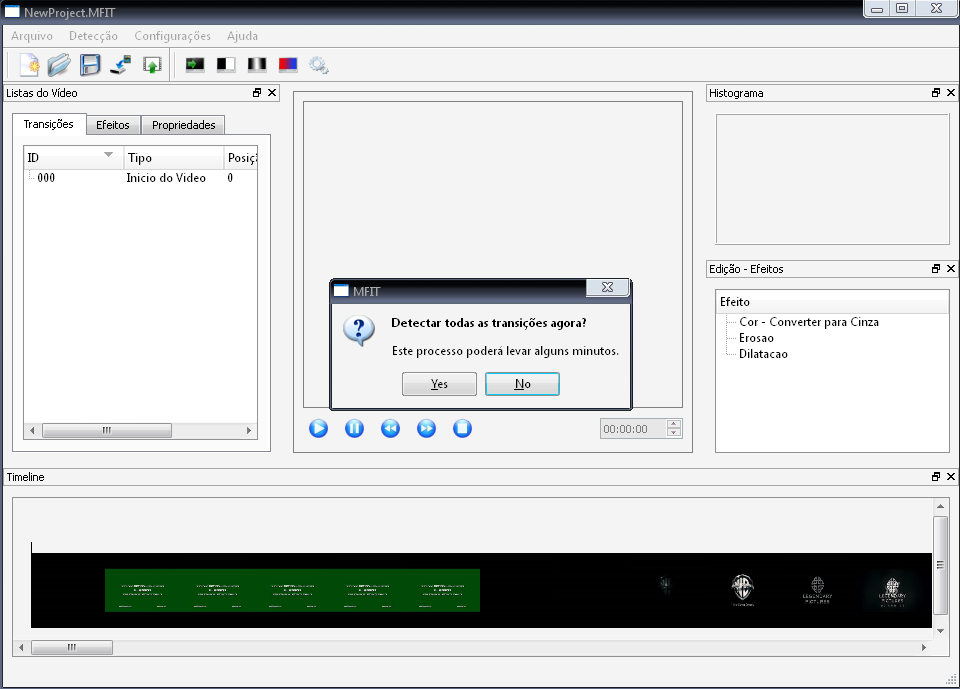
\includegraphics[width=0.7\linewidth]{imagens/carregar4.png}
 \caption{V�deo carregado e janela questionando o processo de detec��o.}
 Fonte: Autor.
 \label{img:carregar4}
\end{figure}

\item{Processo finalizado, o V�deo est� pronto para se efetuar todas as opera��es poss�veis (Figura \ref{img:carregar5}). }

\begin{figure}[h|top]
 \centering
 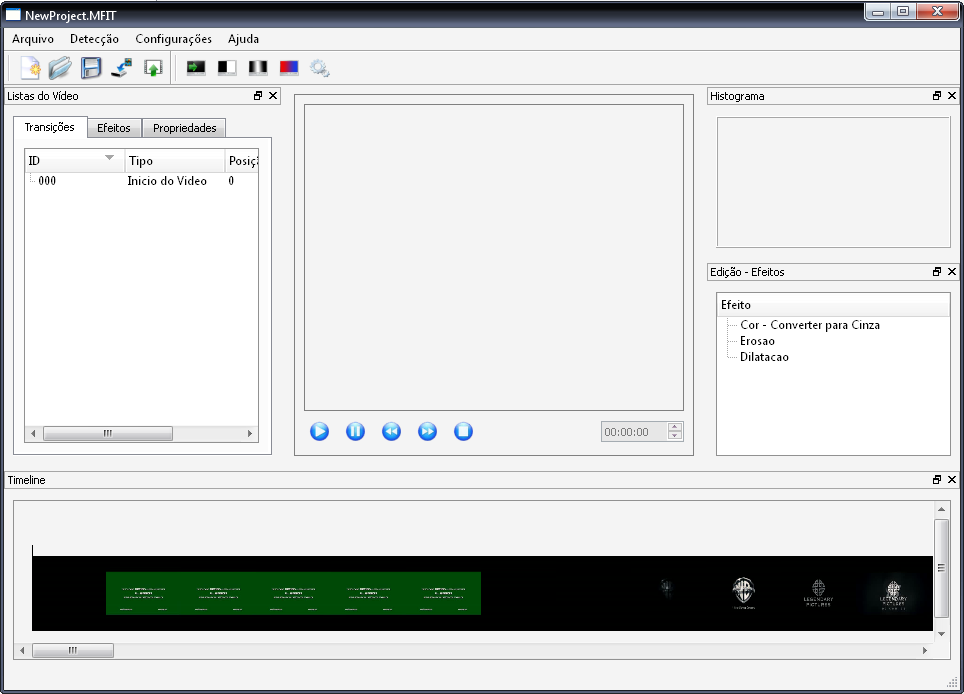
\includegraphics[width=0.7\linewidth]{imagens/carregar5.png}
 \caption{Fim do processo.}
 Fonte: Autor.
 \label{img:carregar5}
\end{figure}

\end{enumerate}

\section{Detec��o de transi��es\label{carrega_video}}

\hspace{1.25cm}Nesta se��o detalharemos os passos necess�rios para
se detectar as transi��es de um V�deo.

\hspace{0.65cm}Para esta funcionalidade temos dois caminhos:

\begin{enumerate}
\item{� partir do carregamento do V�deo}

\subitem{ Ao chegar no passo 4 do processo de carregamento de V�deo
(Se��o \ref{carrega_video}), existe a op��o de aceitar a detec��o de
todas as transi��es. Para isso, basta clicar em ``OK'' quando o
sistema questionar sobre a detec��o. Com isso o processo de detec��o
de todas as transi��es se iniciar�. ( Figura \ref{img:carregar4} )}

\item{Ap�s o carregamento do V�deo}

\subitem{ Ap�s realizar todos os passos do processo de carregamento do V�deo (Se��o \ref{carrega_video}),
os bot�es de detec��o de transi��o estar�o habilitados. Escolha a detec��o que deseja e pressione o bot�o (Figura \ref{img:carregar5} )}

\item{ Ap�s escolher um dos passos acima, o sistema realizar� a detec��o de transi��es, com isso as transi��es ficar�o delimitadas
na Timeline, e a lista de transi��es ser� preenchida (Figura
\ref{img:transicoes1}).}

\end{enumerate}

\begin{figure}[h|top]
 \centering
 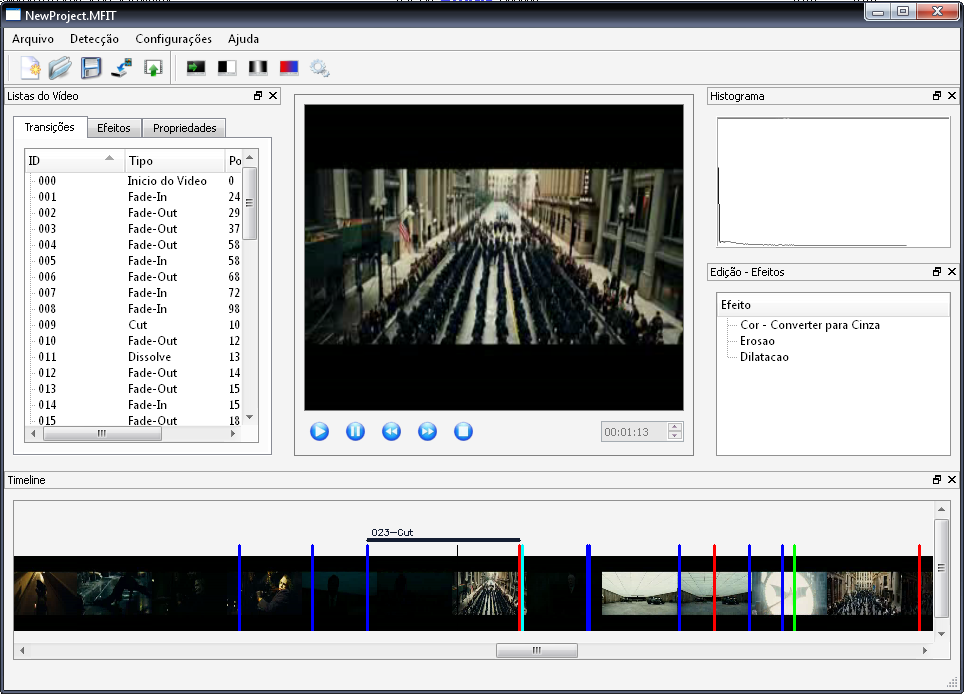
\includegraphics[width=0.8\linewidth]{imagens/transicoes1.png}
 \caption{Transi��es Detectadas.}
 Fonte: Autor.
 \label{img:transicoes1}
\end{figure}

\section{Configura��es da Detec��o \label{config_detecta}}

\hspace*{1.25cm}Para realizar a detec��o de transi��es, o usu�rio
tem como op��o alterar algumas configura��es com o intuito de
melhorar a performance da detec��o.

\hspace{0.65cm}A Figura \ref{img:configuracoes} mostra a janela de
configura��es que � mostrada quando o usu�rio acessa o menu de
configura��es.

\begin{figure}[h|top]
 \centering
 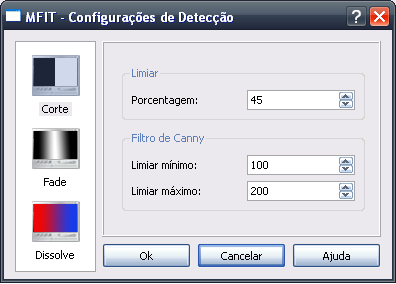
\includegraphics[width=0.8\linewidth]{imagens/configuracoes.png}
 \caption{Janela de configura��es.}
 Fonte: Autor.
 \label{img:configuracoes}
\end{figure}

\hspace*{0.65cm}No canto esquerdo desta janela, encontra-se um menu
que d� acesso �s configura��es espec�ficas pra cada tipo de
transi��o. No entanto s� est�o dispon�veis nesta vers�o, as
configura��es para detec��o do tipo corte.

\hspace*{0.65cm}Cada item � explicado a seguir:

\begin{enumerate}

\item{\textbf{Porcentagem:}
Aqui � poss�vel alterar o valor do limiar para defini��o de quais
bordas geradas atrav�s da aplica��o do Filtro de Canny sobre o Ritmo
Visual ser�o consideradas cortes. O valor aqui definido corresponde
� porcentagem da altura do Frame. Portanto quanto maior for esta
porcentagem, maiores dever�o ser as bordas para que sejam
consideradas cortes. Recomenda-se n�o utilizar valores muito baixos
para que a quantidade de falsas detec��es aumente.}

\item{\textbf{Limiar M�nimo:}
Este limiar corresponde ao limiar mais baixo para o processo de
limiariza��o dupla, ou histerese. Quanto mais baixo for este limiar,
maior ser� o n�mero de bordas detectadas, causando um aumento do
n�mero de falsas detec��es. No entanto, para cada tipo de v�deo h�
uma configura��o que ir� gerar resultados mais satisfat�rios.}

\item{\textbf{Limiar M�ximo:}
Este limiar corresponde ao limiar mais alto para o processo de
limiariza��o dupla, ou histerese. Seu comportamento � semelhante ao
do limiar m�nimo, sendo que para cada tipo de v�deo h� uma
configura��o que gera melhores resultados.}

\end{enumerate}

\section{Aplica��o de Efeito\label{carrega_video}}

\hspace{1.25cm}Nesta se��o ser�o detalhados os passos necess�rios
para se aplicar um efeito no V�deo.

\hspace{0.65cm}Como pr�-requisito necessitamos de um V�deo
carregado.

\begin{enumerate}

\item{Com o V�deo aberto, selecione um dos efeitos da lista de efeitos a direita (Figura \ref{img:efeitos1})}

\begin{figure}[h|top]
 \centering
 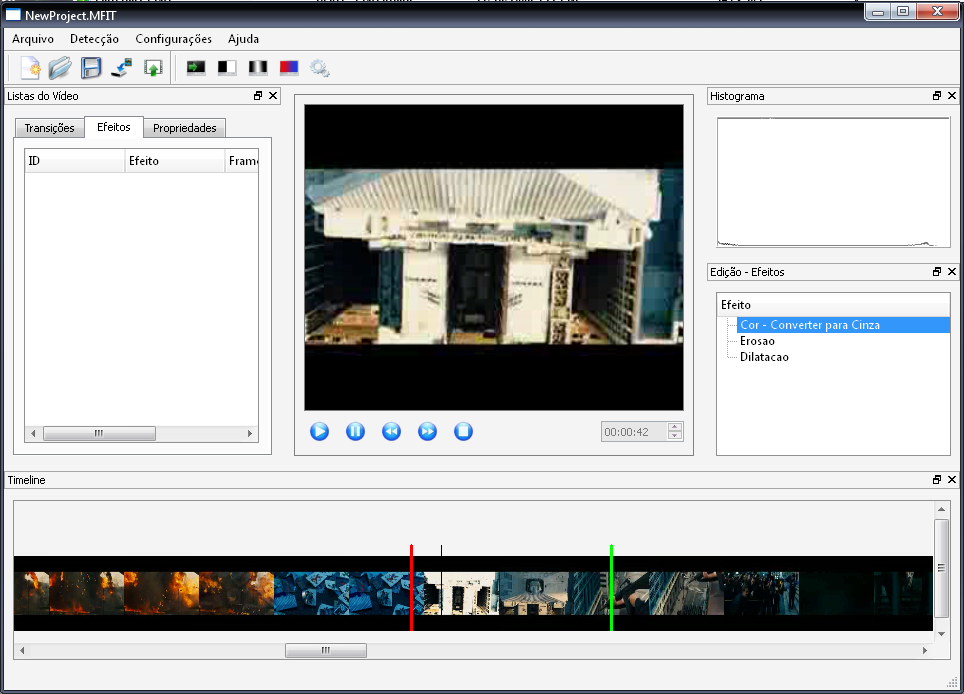
\includegraphics[width=0.7\linewidth]{imagens/efeitos1.png}
 \caption{Lista de Efeitos.}
 Fonte: Autor.
 \label{img:efeitos1}
\end{figure}

\item{Para aplicar o efeito, clique no efeito desejado e arraste para a posi��o o v�deo. Note que o sistema sinalizar�
    as transi��es onde este efeito ser� aplicado .(Figura \ref{img:efeitos2})}

\begin{figure}[h|top]
 \centering
 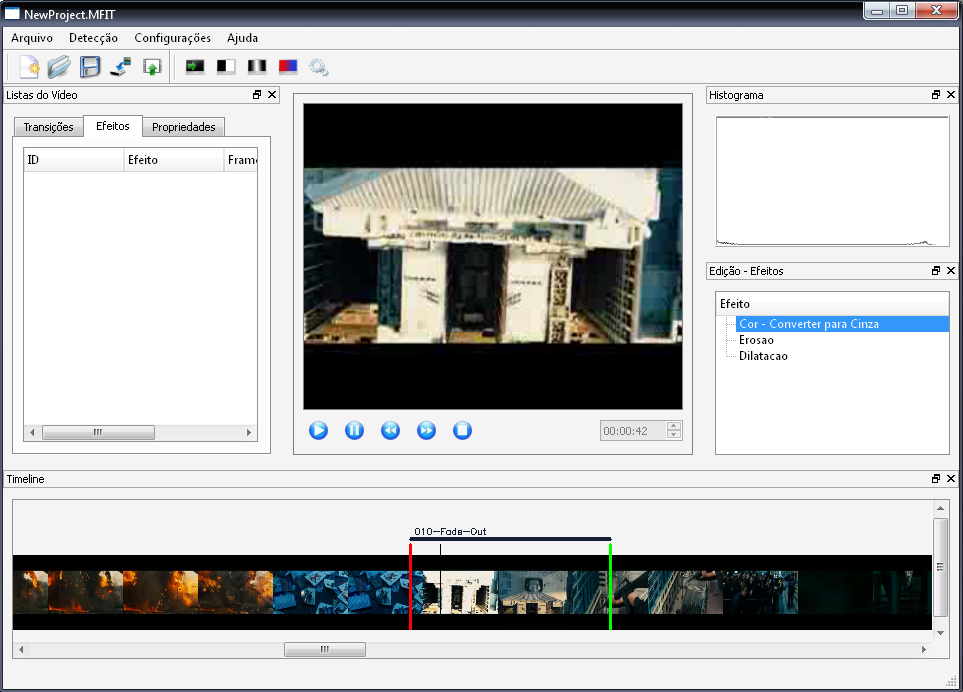
\includegraphics[width=0.7\linewidth]{imagens/efeitos2.png}
 \caption{Arrastando o efeito desejado.}
 Fonte: Autor.
 \label{img:efeitos2}
\end{figure}

\item{Caso o desejado seja aplicar em v�rias transi��es, no momento que estiver arrastando, segure a tecla CTRL (Figura \ref{img:efeitos3}).}

\begin{figure}[h|top]
 \centering
 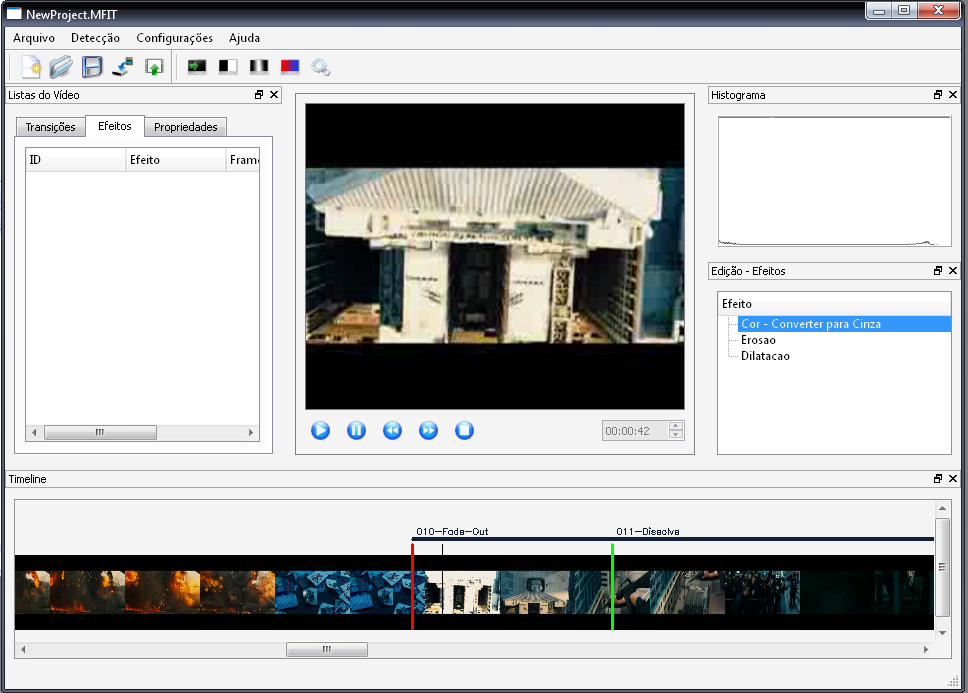
\includegraphics[width=0.7\linewidth]{imagens/efeitos3.png}
 \caption{Arrastando para m�ltiplas transi��es.}
 Fonte: Autor.
 \label{img:efeitos3}
\end{figure}

\item{Com isso o efeito vai ser aplicado no intervalo de transi��es desejados, note que a lista de efeitos conta agora com uma entrada, e a visualiza��o
    do v�deo j� contem o efeito aplicado (Figura \ref{img:efeitos4})}

\begin{figure}[h|top]
 \centering
 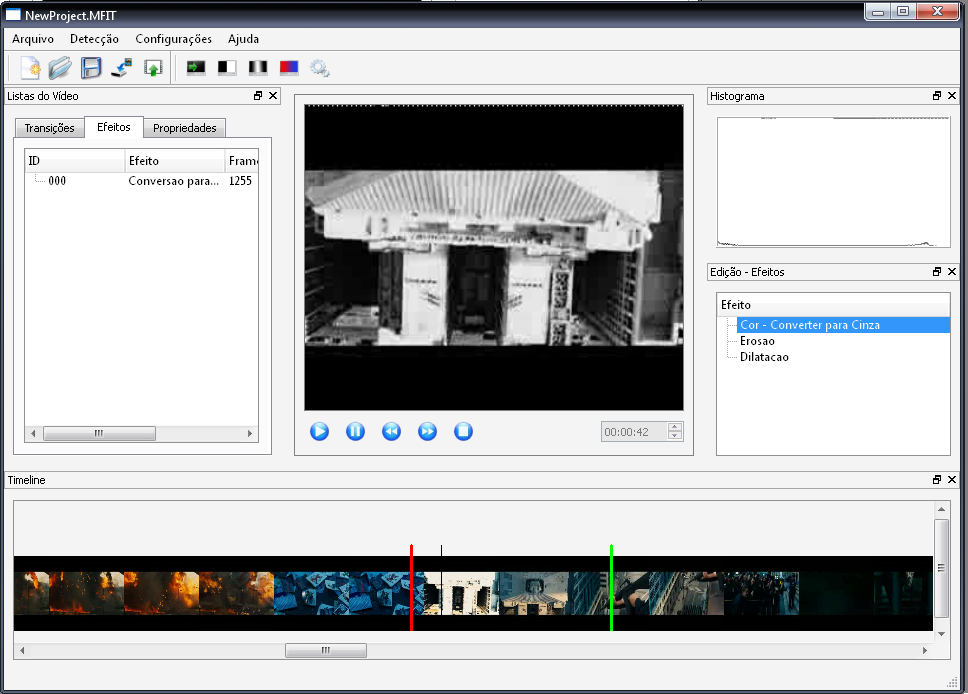
\includegraphics[width=0.7\linewidth]{imagens/efeitos4.png}
 \caption{Efeito aplicado.}
 Fonte: Autor.
 \label{img:efeitos4}
\end{figure}

\end{enumerate}

\section{Renderizar V�deo\label{carrega_video}}

\hspace{1.25cm}Nesta se��o detalharemos os passos necess�rios para
se renderizar o V�deo.

\hspace{0.65cm}Como pr�-requisito temos que ter um V�deo carregado.

\begin{enumerate}

\item{Ap�s aplicarmos efeitos em um V�deo, � hora de renderiza-lo para verificarmos o resultado final.
    Clique na op��o ``Renderizar'' do menu ``Arquivo'' (Figura \ref{img:render1})}

\begin{figure}[h|top]
 \centering
 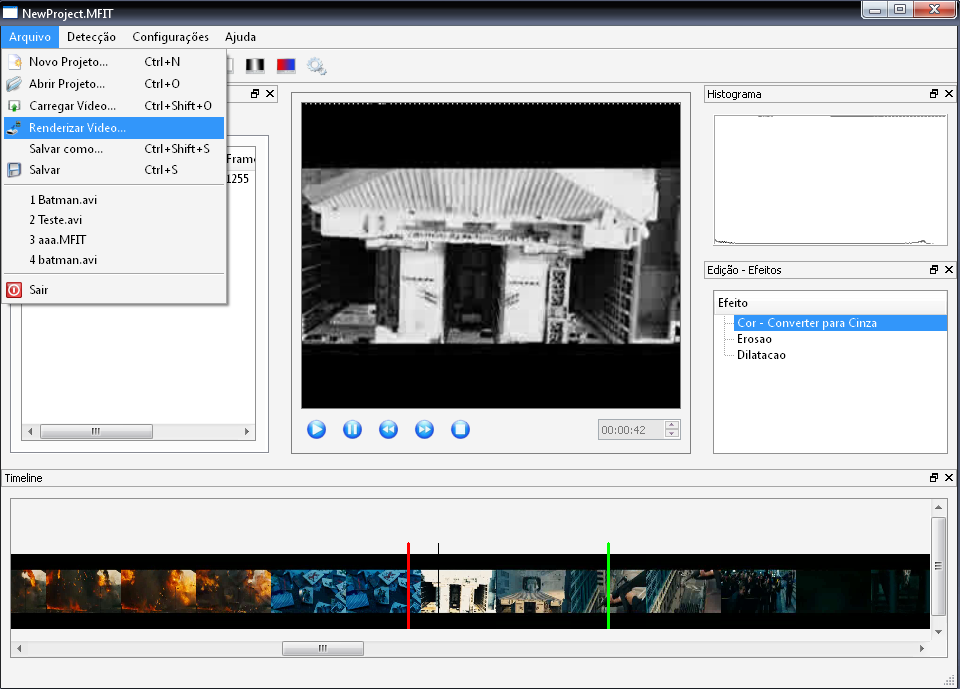
\includegraphics[width=0.7\linewidth]{imagens/render1.png}
 \caption{Op��o ``Renderizar'' do menu ``Arquivo''.}
 Fonte: Autor.
 \label{img:render1}
\end{figure}

\item{Na janela que se abriu, selecione um nome para o V�deo e pressione ``OK'' (Figura \ref{img:render2})}

\begin{figure}[h|top]
 \centering
 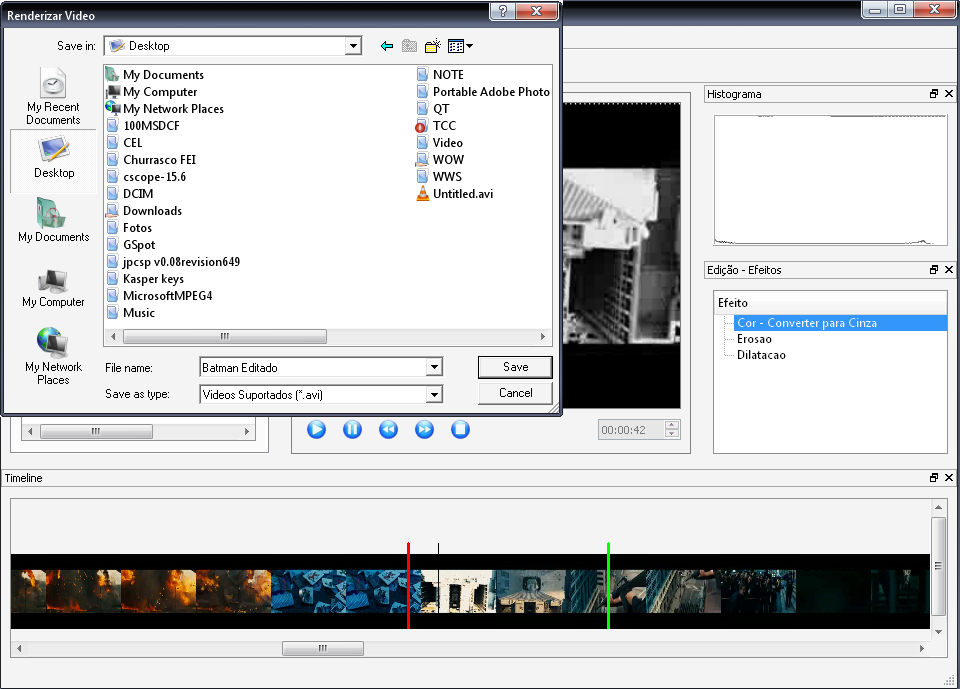
\includegraphics[width=0.7\linewidth]{imagens/render2.png}
 \caption{Janela de escolha do nome do V�deo.}
 Fonte: Autor.
 \label{img:render2}
\end{figure}

\item{Por fim, quando o MFIT voltar para sua janela principal, o video j� estar� salvo no local selecionado (Figura \ref{img:render3})}

\begin{figure}[h|top]
 \centering
 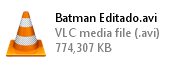
\includegraphics[width=0.3\linewidth]{imagens/render3.png}
 \caption{V�deo renderizado.}
 Fonte: Autor.
 \label{img:render3}
\end{figure}

\end{enumerate}

\section{Editar Transi��o\label{carrega_video}}

\hspace{1.25cm}Nesta se��o detalharemos os passos necess�rios para
se editar uma Transi��o.

\hspace{0.65cm}Como pr�-requisito temos que ter um V�deo carregado,
e suas transi��es detectadas.

\begin{enumerate}

\item{De um duplo clique na transi��o desejada, uma nova janela se abrir� (Figura \ref{img:edit1})}

\begin{figure}[h|top]
 \centering
 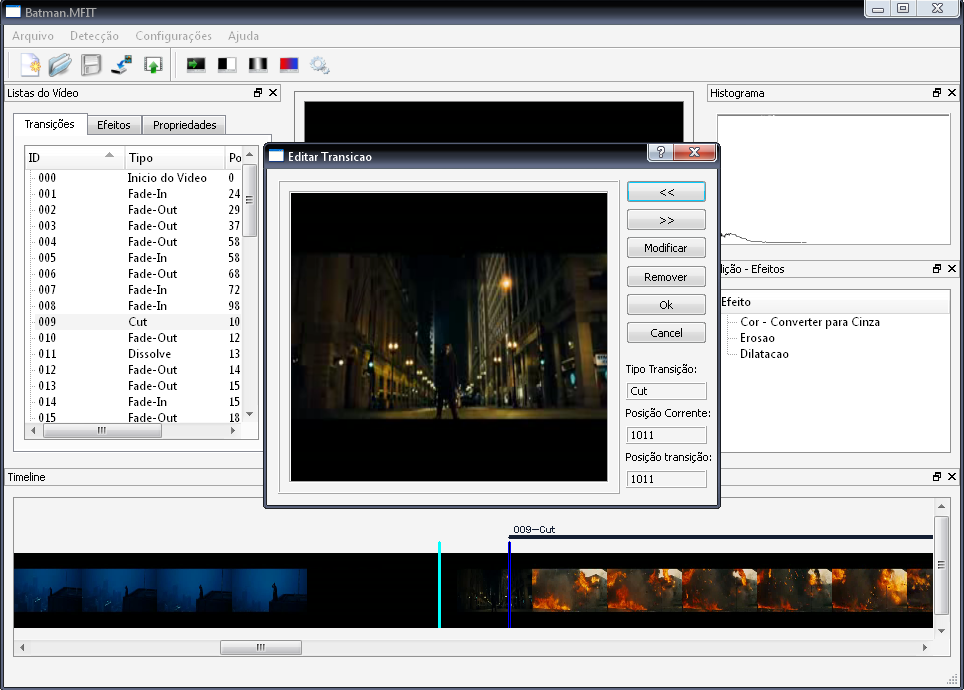
\includegraphics[width=0.7\linewidth]{imagens/edit1.png}
 \caption{Janela de edi��o de transi��es.}
 Fonte: Autor.
 \label{img:edit1}
\end{figure}

\item{Para modificar o ponto da transi��o:}
\subitem{Clique nos bot�es ``$<<$'' ou ``$>>$'' para navegar no v�deo (Figura \ref{img:edit2})}

\begin{figure}[h|top]
 \centering
 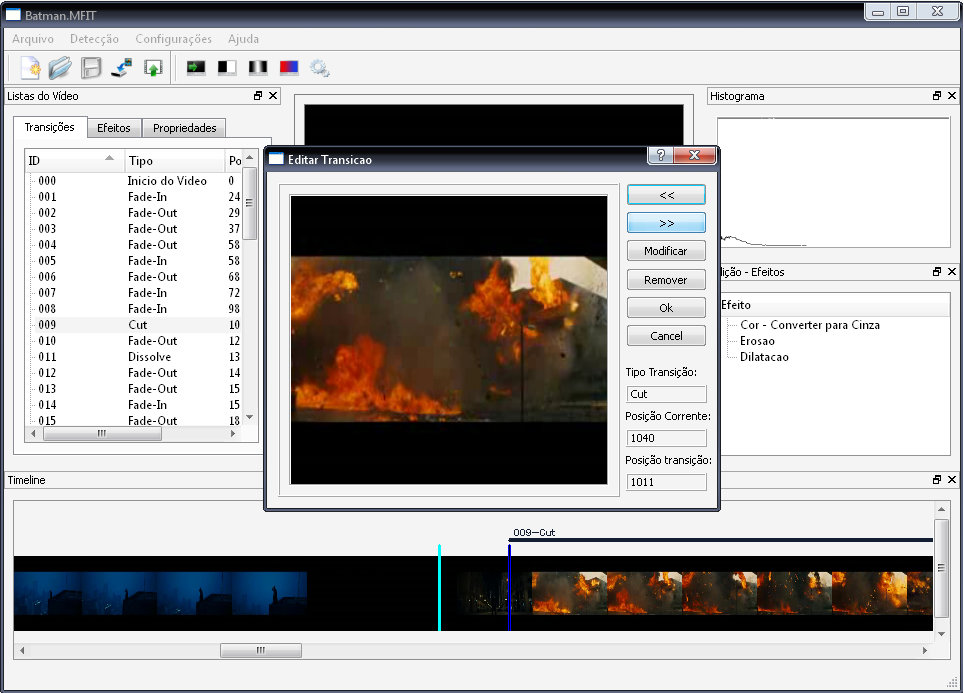
\includegraphics[width=0.7\linewidth]{imagens/edit2.png}
 \caption{Navegando no V�deo.}
 Fonte: Autor.
 \label{img:edit2}
\end{figure}

\subitem{No momento em que desejar definir a posi��o corrente como a
posi��o da transi��o, clique em ``Modificar'' (Figura
\ref{img:edit3}). Note que o valor da ``Posi��o Transi��o'' assumir�
o valor da ``Posi��o Corrente''.}

\begin{figure}[h|top]
 \centering
 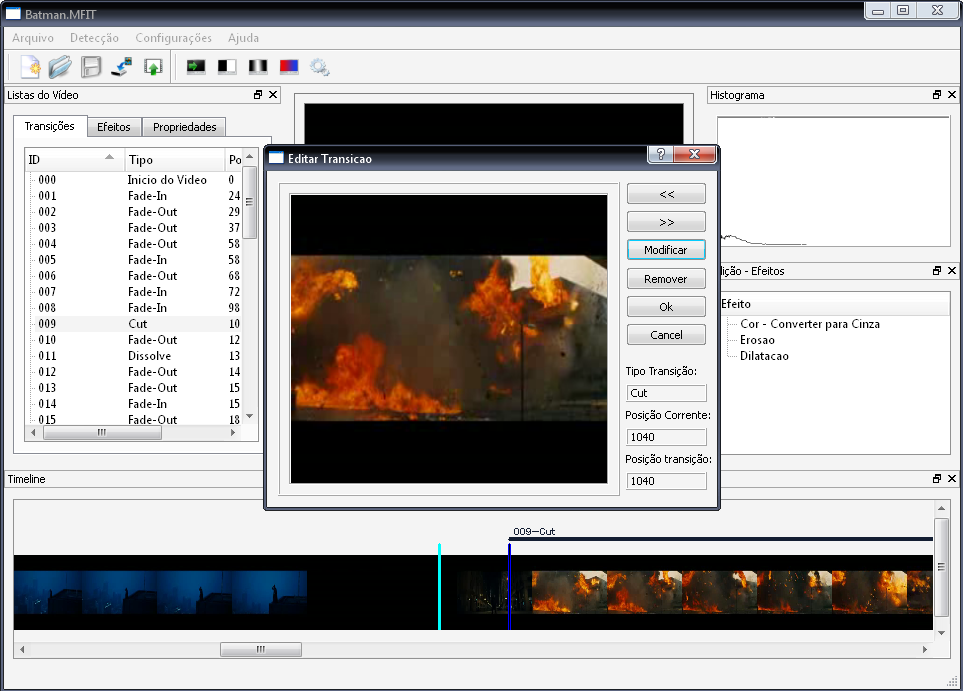
\includegraphics[width=0.7\linewidth]{imagens/edit3.png}
 \caption{Modificando a posi��o da transi��o.}
 Fonte: Autor.
 \label{img:edit3}
\end{figure}

\subitem{Clique em ``Ok'' para confirmar as altera��es.}

\item{Para remover o da transi��o:}
\subitem{Clique no bot�o ``Remover'' }
\subitem{Clique em ``Ok'' para confirmar as altera��es}

\item{Ap�s clicar em ``Ok'', o sistema aplicar� as altera��es.
Na Figura \ref{img:edit4} removemos a transi��o selecionada, e na Figura \ref{img:edit5}, modificamos seu ponto de ocorr�ncia.}

\begin{figure}[h|top]
 \centering
 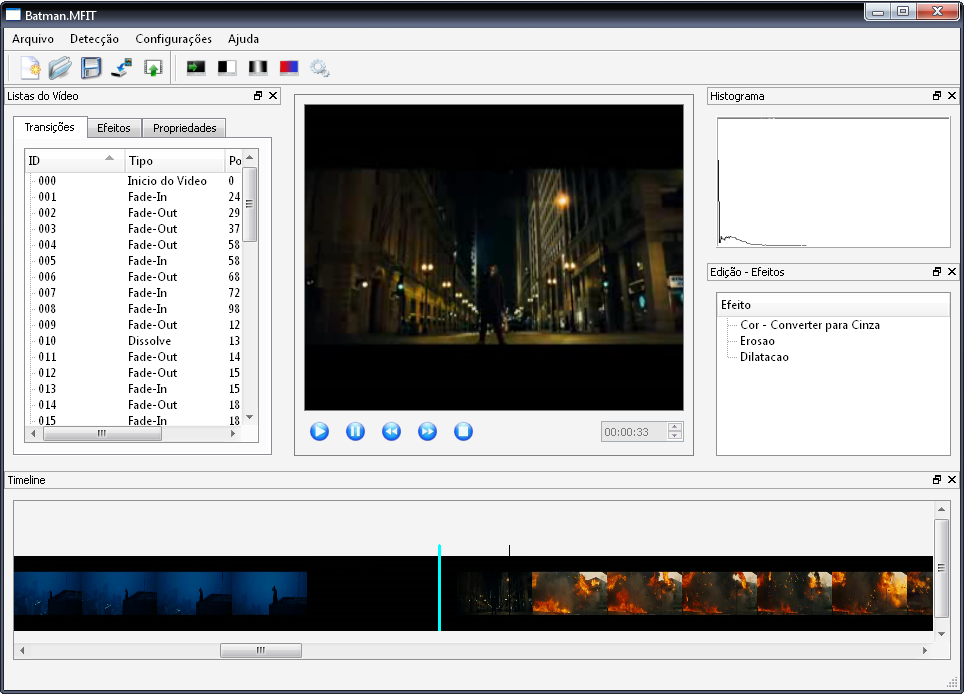
\includegraphics[width=0.7\linewidth]{imagens/edit4.png}
 \caption{Transi��o Removida.}
 Fonte: Autor.
 \label{img:edit4}
\end{figure}

\begin{figure}[h|top]
 \centering
 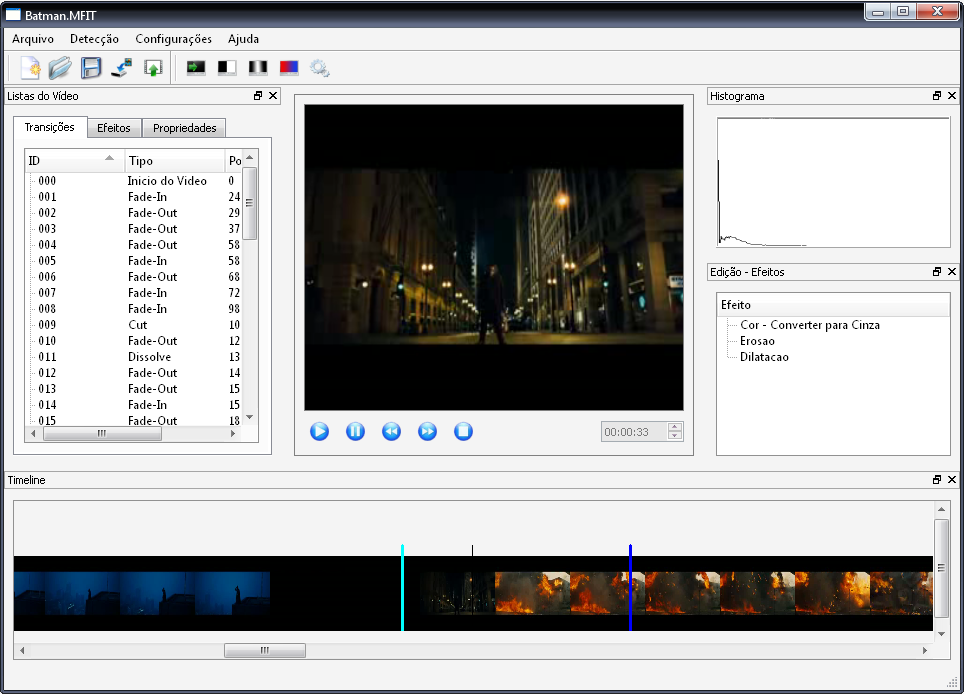
\includegraphics[width=0.7\linewidth]{imagens/edit5.png}
 \caption{Ponto da Transi��o modificado.}
 Fonte: Autor.
 \label{img:edit5}
\end{figure}

\end{enumerate}


\end{spacing}

\appendix

%\include{apendice}

%Bibliografia
\begin{spacing}{1.0}
\bibliographystyle{apalike}
%\bibliographystyle{abbrv}
\bibliography{referencias}
\end{spacing}

\end{document}
